%% Autor: Björn Ritterbecks 
%% Letzte Aenderung: 15.06.2016 
\thisfloatsetup{%
  capbesidewidth=\marginparwidth}
\begin{figure}[htbp]
\vspace*{0.2cm}
\centering
%\sansmath
 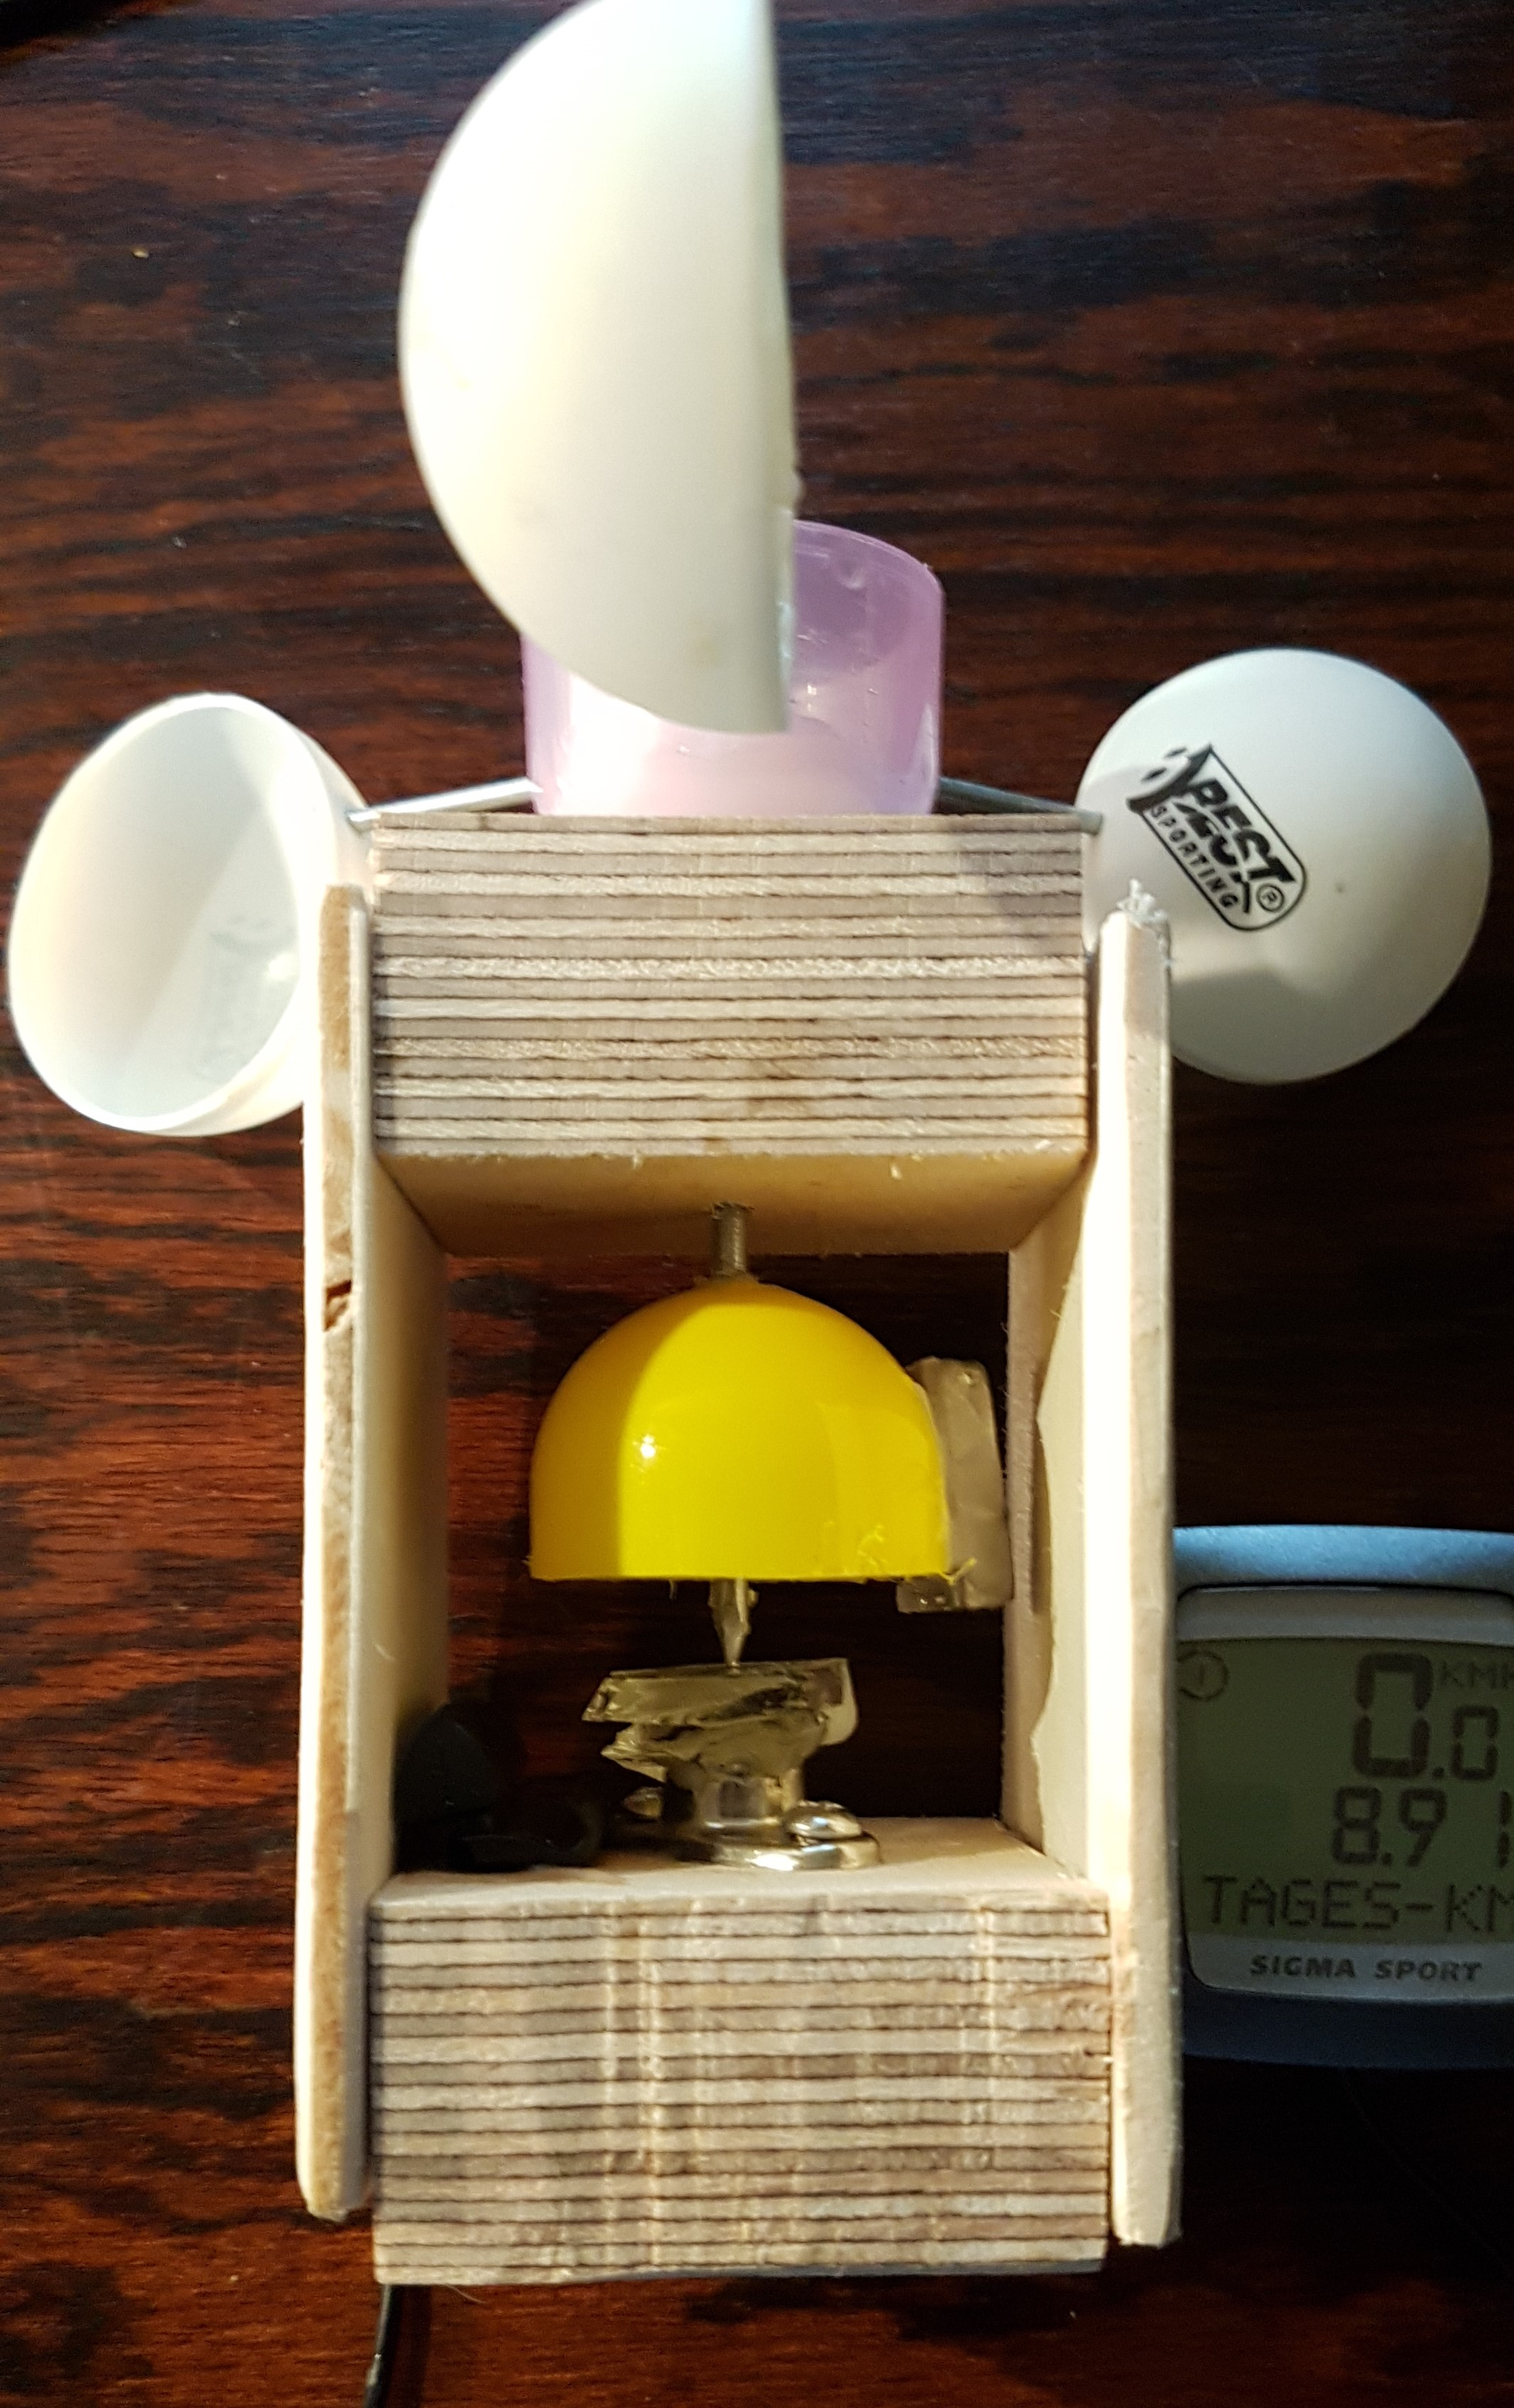
\includegraphics[width=0.75\textwidth]{images/Windkraft.jpg}
  \caption[Selbstbau eines Anemometers]{Aus einfachen Materialien und einem Fahrradcomputer gebautes Anemometer. Die Idee hinter dem Funktionsprinzip kommt von \textsc{Rüdiger Stenzel}: \url{http://www.dc4fs.de/wetter/anemo.htm}. Die Tischtennisballhälften drehen sich bei einem Luftstrom und versetzen damit einen Stahlstift in Rotation, an dem wiederum ein Magnet befestigt ist, der bei jeder Umdrehung durch einen \textsc{Reed-Kontakt} detektiert wird.}
  \label{fig:windgeschw1}
  \vspace{-0pt}
\end{figure}